\documentclass[12pt]{article}

\usepackage{sbc-template}
\usepackage{graphicx,url}
\usepackage[utf8]{inputenc}
\usepackage[brazil]{babel}
%\usepackage[latin1]{inputenc}  

     
\sloppy

\title{Perfil de desempenho e oportunidades de otimização da implementação do método CSEM 3D}

\author{Rômulo T. Lima\inst{1,2}, Mateus F. Lima de Souza\inst{1,3}}

\address{  Laboratório Nacional de Computação Científica (LNCC)\\
  Getúlio Vargas Av., 333, Quitandinha Petrópolis - RJ - Brasil
\nextinstitute
Universidade Católica de Petrópolis (UCP)\\
  R. Barão do Amazonas, 124 - Centro, Petrópolis - RJ - Brasil
\nextinstitute
  Centro Federal de Educação Tecnológica Celso Suckow da Fonseca (CEFET-FR) \\
  R. Gen. Canabarro, 485 - Maracanã, Rio de Janeiro - RJ - Brasil
  \email{\{romulotl,facanha\}@lncc.br}
}

\begin{document} 

\maketitle

\begin{abstract}
  This meta-paper describes the style to be used in articles and short papers
  for SBC conferences. For papers in English, you should add just an abstract
  while for the papers in Portuguese, we also ask for an abstract in
  Portuguese (``resumo''). In both cases, abstracts should not have more than
  10 lines and must be in the first page of the paper.
\end{abstract}
     
\begin{resumo} 
  Este meta-artigo descreve o estilo a ser usado na confecção de artigos e
  resumos de artigos para publicação nos anais das conferências organizadas
  pela SBC. É solicitada a escrita de resumo e abstract apenas para os artigos
  escritos em português. Artigos em inglês deverão apresentar apenas abstract.
  Nos dois casos, o autor deve tomar cuidado para que o resumo (e o abstract)
  não ultrapassem 10 linhas cada, sendo que ambos devem estar na primeira
  página do artigo.
\end{resumo}


\section{Introdução}

%\subsection{CSEM} \label{sec:firstpage}
Métodos Eletromagnéticos de Fonte Controlada (CSEM) é uma técnica geofísica usada para explorar o subsolo da Terra em busca de reservas de petróleo e gás, bem como de outros recursos minerais.

A técnica envolve o uso de uma fonte eletromagnética para produzir um sinal de baixa frequência, que é então detectado por sensores colocados no fundo do mar ou em terra. O sinal pode penetrar nas camadas da Terra e interagir com qualquer material condutor, como rochas contendo hidrocarbonetos, criando um campo eletromagnético secundário que é medido pelos sensores.

Ao analisar a resposta do campo secundário, os geofísicos podem criar um modelo 3D da subsuperfície, que pode ser usado para identificar a localização e o tamanho de potenciais reservas de hidrocarbonetos e outras características geológicas.

O CSEM é particularmente útil para exploração em áreas offshore, onde os métodos sísmicos podem ser menos eficazes devido à presença de hidratos de gás ou outros fatores. No entanto, também pode ser usado com outras técnicas geofísicas, como levantamentos sísmicos, para fornecer uma compreensão mais abrangente da subsuperfície.

%\section{Metodologia}

%\subsection{HPCToolkit}
HPCToolkit~\cite{hpctoolkit2010} é um conjunto de ferramentas de análise de desempenho de código-fonte aberto projetado para ajudar os desenvolvedores a entender e otimizar o desempenho de seus aplicativos em sistemas de computação de alto desempenho (HPC, do termo em inglês High-Performance Computing), e fornece uma ampla gama de recursos para análise de desempenho, incluindo-se:
\begin{itemize}
 \item Coleta de dados de desempenho: o HPCToolkit pode coletar dados de desempenho durante a execução do programa, incluindo informações sobre o tempo de CPU, eventos de hardware, alocação de memória e outros dados relevantes para a análise de desempenho.
  \item Análise de dados: o HPCToolkit pode analisar os dados de desempenho coletados para identificar gargalos de desempenho e oportunidades de otimização.
 \item Visualização de dados: o HPCToolkit pode visualizar os dados de desempenho coletados em vários formatos.
\end{itemize}
O HPCToolkit suporta várias linguagens de programação, tais como C, C++ e Fortran, e é compatível com diferenes arquiteturas de hardware, como CPUs, GPUs e clusters de computadores.

\section{Resultados}

\subsection{Estudo de caso}
\subsection{Recursos computacionais}
\begin{figure}
\centering
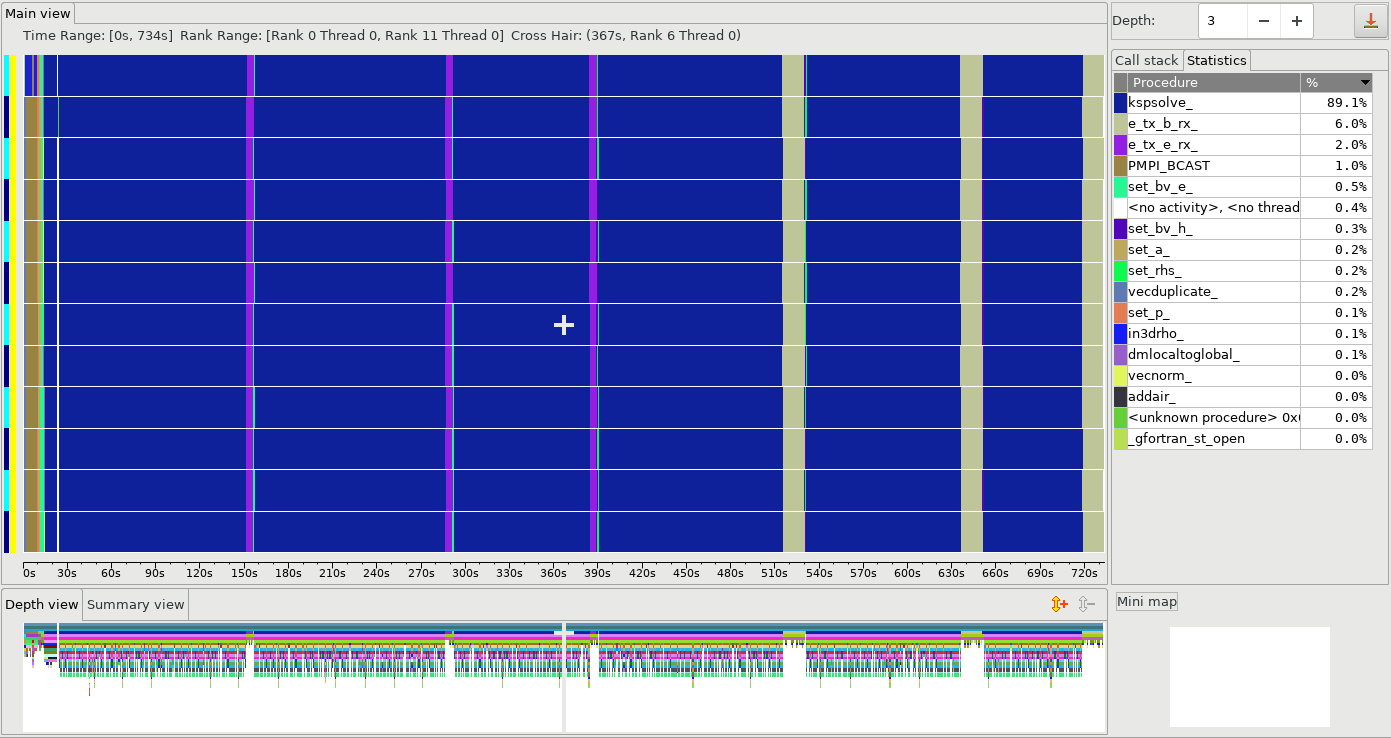
\includegraphics[width=.5\textwidth]{figures/openmpi/Nodes1_MPI12.png}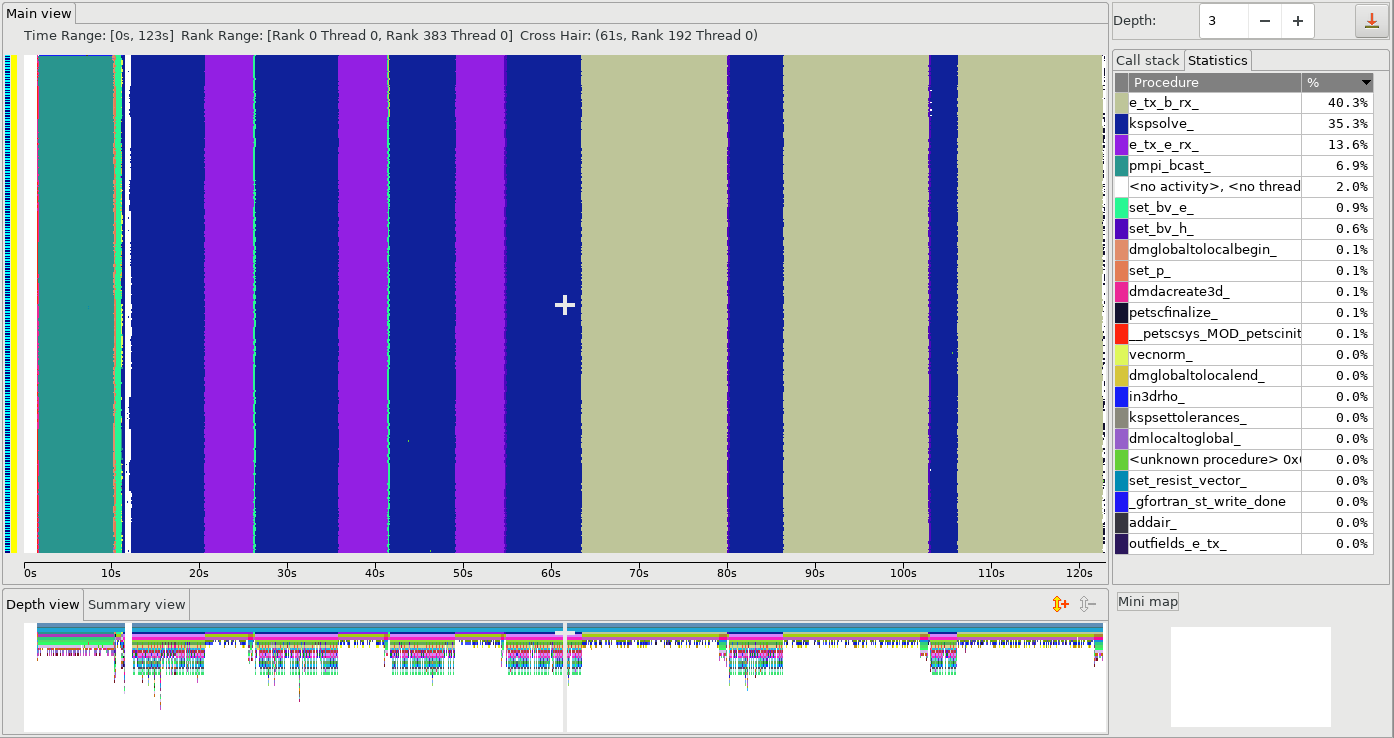
\includegraphics[width=.5\textwidth]{figures/openmpi/Nodes16_MPI384.png}
\caption{HPCToolkit.}
\label{fig:nodes1mpi12}
\end{figure}

% \begin{figure}
% \centering
% 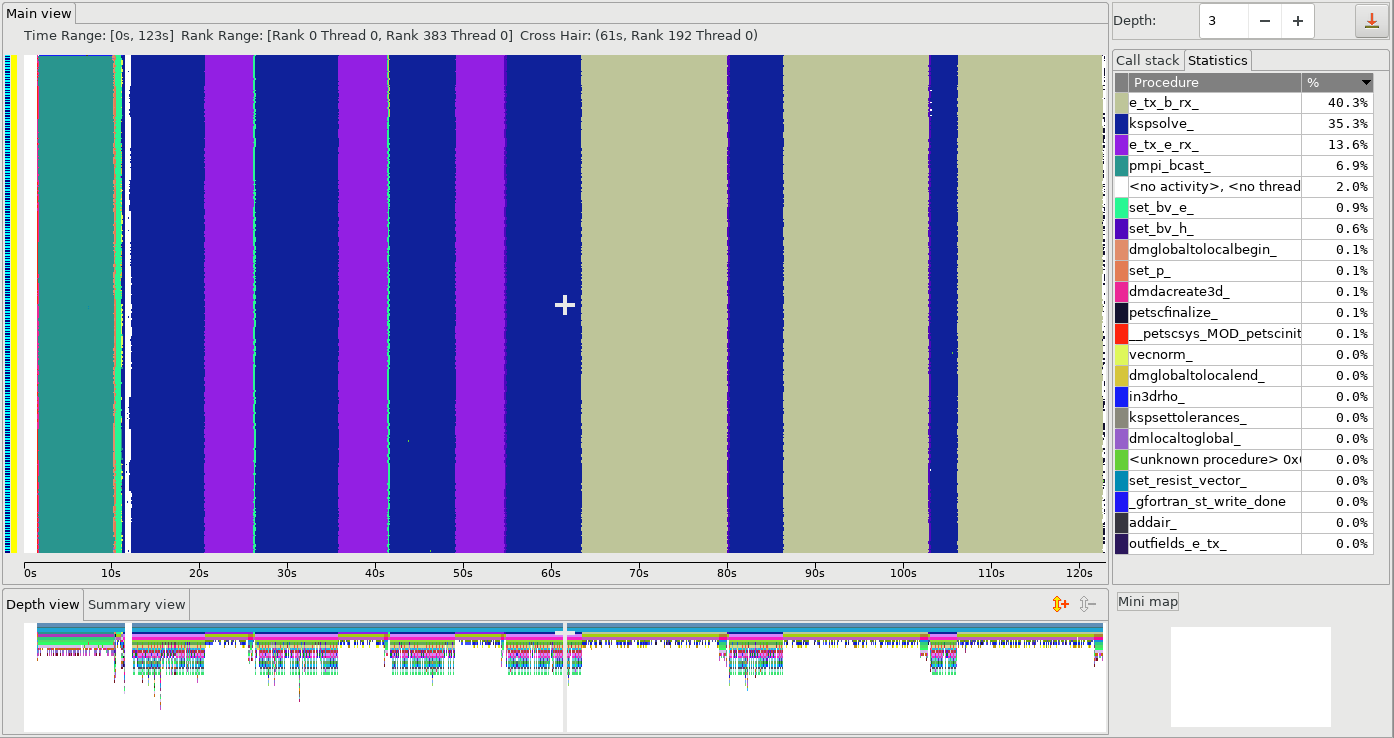
\includegraphics[width=.5\textwidth]{figures/openmpi/Nodes16_MPI384.png}
% \caption{HPCToolkit.}
% \label{fig:nodes16mpi384}
% \end{figure}

\begin{figure}
\centering
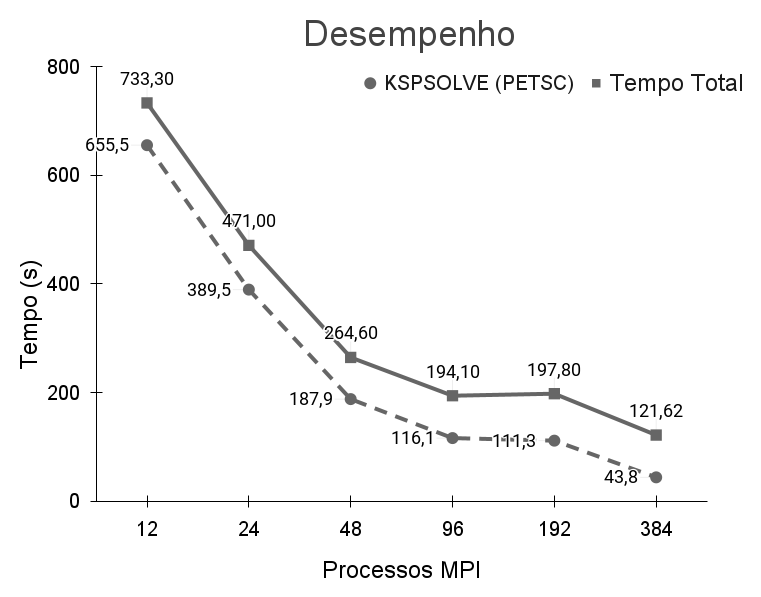
\includegraphics[width=.5\textwidth]{figures/openmpi/desempenho.png}
\caption{Desempenho}
\label{fig:desempenho}
\end{figure}




\section{Comentários Finais}


\section{Agradecimentos}
os autores agradecem ao Laboratório Nacional de Computação Científica (LNCC/MCTI) por fornecer recursos HPC do supercomputador SDumont, que contribuíram para os resultados da pesquisa relatados neste artigo. URL: http://sdumont.lncc.br
\section{References}

\bibliographystyle{sbc}
\bibliography{sbc-template}

\end{document}
